\newpage
\subsection{Khôi phục tài khoản}

\subsubsection*{Mục tiêu}
Chức năng khôi phục tài khoản cho phép người dùng đặt lại mật khẩu (passphrase) khi không còn nhớ mật khẩu cũ. Khác với đặt lại mật khẩu thông thường, hệ thống vẫn đảm bảo khôi phục được private key đã mã hóa trước đó – nhờ sử dụng một \textbf{recovery code} (AES key phụ) đã được lưu trữ an toàn từ khi đăng ký.

\subsubsection*{Giao diện}
Giao diện khôi phục gồm 2 bước:
\begin{itemize}
    \item \textbf{Bước 1:} Người dùng nhập email và recovery code để xác minh quyền sở hữu tài khoản.
    \begin{figure}[H]
        \centering
        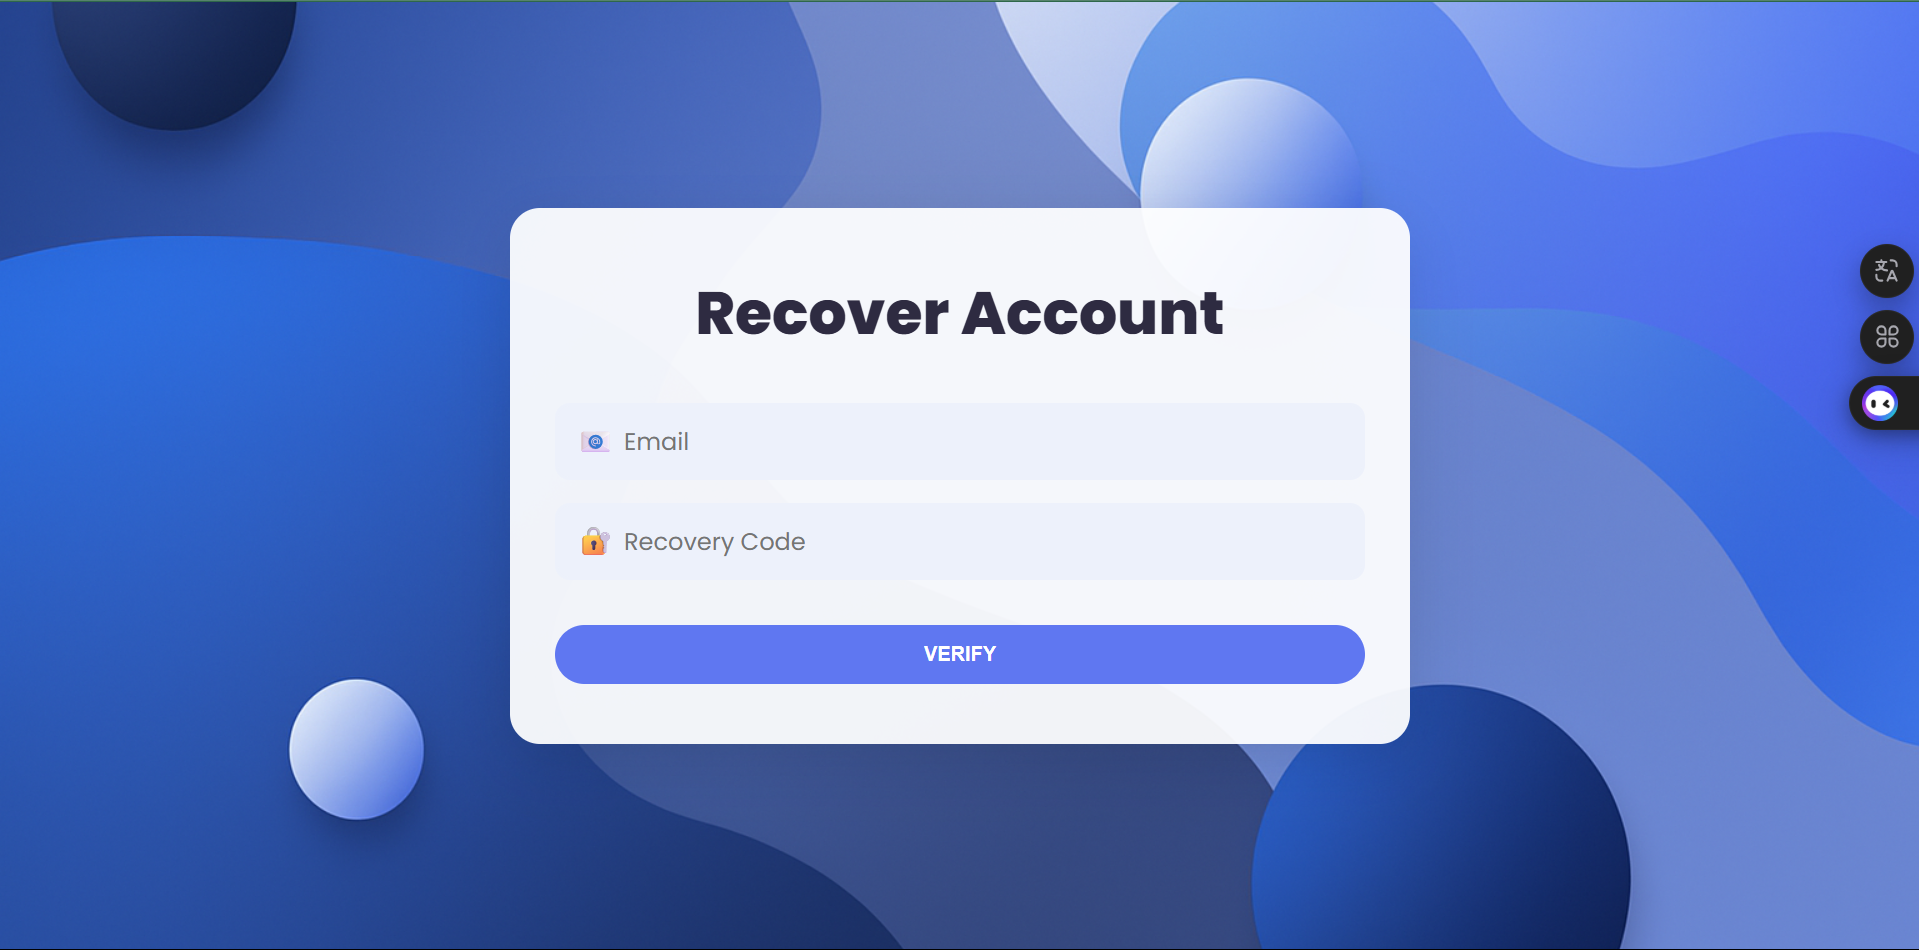
\includegraphics[width=0.85\textwidth]{img/17_recover/17_recover_recovery_code.png}
        \caption{Nhập mã khôi phục}
    \end{figure}

    \item \textbf{Bước 2:} Nếu thành công, hệ thống cho phép nhập mật khẩu mới (passphrase), sau đó sẽ mã hóa lại khóa riêng và recovery key.
    \begin{figure}[H]
        \centering
        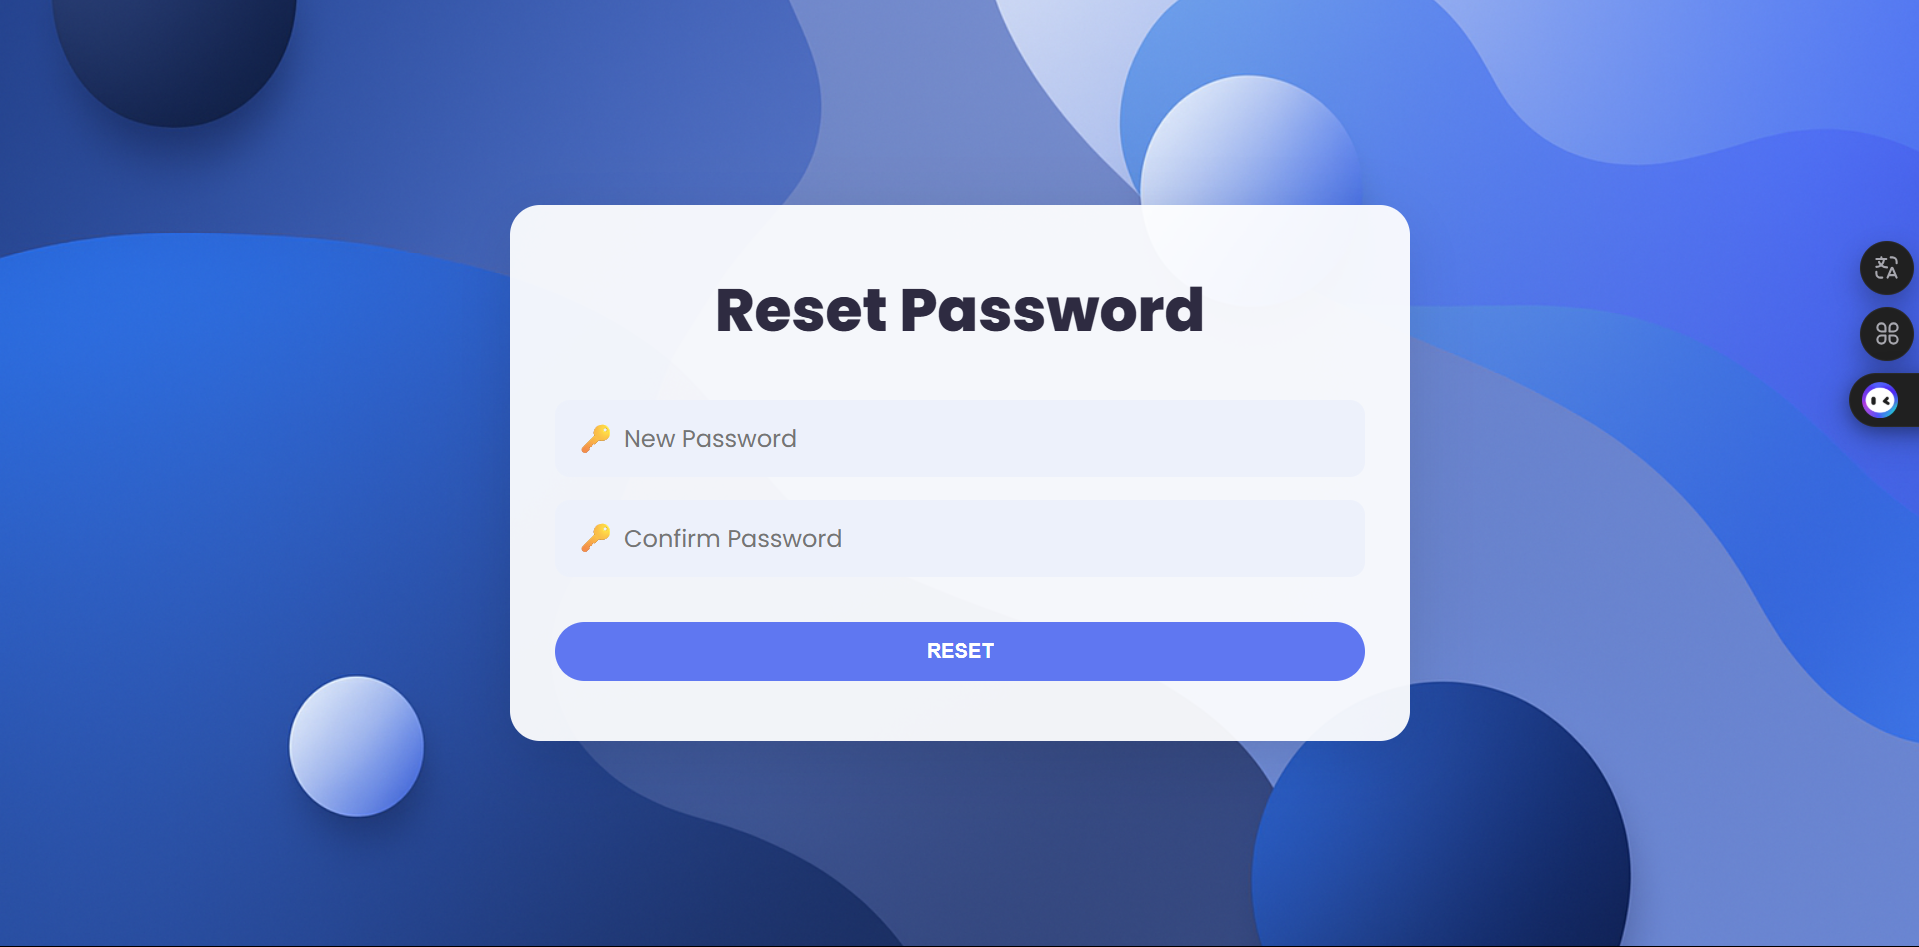
\includegraphics[width=0.85\textwidth]{img/17_recover/17_recovery_pw.png}
        \caption{Nhập mật khẩu mới}
    \end{figure}
\end{itemize}

\subsubsection*{Quy trình thực hiện}
\begin{description}

    \item[\textbf{Bước 1 - Xác minh recovery code}]
    \begin{itemize}
        \item Người dùng nhập recovery code → hệ thống derive AES key từ recovery code đó.
        \item Dùng AES key này để giải mã file \texttt{key\_recovery} chứa private key hiện tại.
        \item Nếu giải mã thành công → recovery code hợp lệ.
    \end{itemize}

    \item[\textbf{Bước 2 - Nhập mật khẩu mới}]
    \begin{itemize}
        \item Người dùng nhập passphrase mới.
        \item Hệ thống mã hóa lại private key hiện tại bằng AES key derive từ passphrase mới.
        \item Đồng thời, mã hóa lại recovery code bằng AES key derive từ passphrase mới → lưu vào cột \texttt{encrypted\_recovery\_code} trong database.
    \end{itemize}

    \item[\textbf{Bước 3 - Cập nhật cơ sở dữ liệu}]
    \begin{itemize}
        \item Hash passphrase mới và cập nhật vào cột \texttt{hashed\_passphrase}.
        \item Ghi log hành động khôi phục với trạng thái thành công hoặc thất bại.
    \end{itemize}
\end{description}

\subsubsection*{Chi tiết kỹ thuật và thư viện bảo mật}
\begin{description}

    \item[\textbf{1. Recovery code}]
    Recovery code là một chuỗi ngẫu nhiên sinh ra khi đăng ký, dùng để derive AES key tạm thời cho mục đích khôi phục khóa.
    \begin{itemize}
        \item Được dùng để giải mã private key hiện tại khi muốn reset password. 
        \item Được mã hóa bằng AES key derive từ passphrase và lưu dưới database.
    \end{itemize}

    \item[\textbf{2. Kiểm tra tính hợp lệ của recovery code}]
    \begin{itemize}
        \item Dùng recovery code derive AES key: \texttt{derive\_aes\_key(recovery\_code)}.
        \item Giải mã file \texttt{key\_recovery} (chứa private key mã hóa) bằng AES key này.
        \item Nếu giải mã được → xác minh thành công.
    \end{itemize}

    \item[\textbf{3. Đặt lại mật khẩu và mã hóa lại dữ liệu}]
    \begin{itemize}
        \item Derive AES key từ passphrase mới.
        \item Mã hóa lại private key bằng AES key mới.
        \item Mã hóa recovery code bằng AES key mới và lưu vào \texttt{encrypted\_recovery\_code}.
        \item Hash passphrase mới với salt → cập nhật vào bảng \texttt{users}.
    \end{itemize}

    \item[\textbf{4. Xử lý lỗi và báo lỗi chi tiết}]
    Hệ thống đảm bảo mọi lỗi trong quá trình khôi phục tài khoản đều được phát hiện, phản hồi rõ ràng cho người dùng, đồng thời ghi log bảo mật để hỗ trợ điều tra.

    \begin{itemize}
        \item \textbf{Thiếu email hoặc recovery code:}
        \begin{itemize}
            \item Nếu không gửi đủ thông tin đầu vào → trả lỗi \texttt{400} với thông báo: \texttt{"Missing recovery information"}.
        \end{itemize}

        \item \textbf{Recovery code không hợp lệ:}
        \begin{itemize}
            \item Nếu recovery code không trùng khớp hoặc giải mã private key thất bại → trả lỗi \texttt{400}, thông báo: \texttt{"Invalid recovery code"}.
            \item Lỗi này thường do nhập sai hoặc đã đổi passphrase trước đó mà chưa cập nhật lại recovery key.
        \end{itemize}

        \item \textbf{Mật khẩu mới không hợp lệ:}
        \begin{itemize}
            \item Nếu passphrase mới không đủ mạnh (dưới 8 ký tự, không có ký tự đặc biệt, chữ hoa, số) → từ chối và trả thông báo cụ thể.
        \end{itemize}

        \item \textbf{Lỗi mã hóa lại private key hoặc recovery key:}
        \begin{itemize}
            \item Nếu trong quá trình mã hóa lại private key bằng passphrase mới xảy ra lỗi → rollback thao tác DB và trả về lỗi \texttt{"Re-encrypt RSA failed"}.
            \item Nếu mã hóa lại recovery key lỗi → báo lỗi \texttt{"Failed to encrypt recovery key"} và không cập nhật thông tin.
        \end{itemize}

        \item \textbf{Lỗi cập nhật CSDL:}
        \begin{itemize}
            \item Nếu xảy ra lỗi khi cập nhật passphrase hoặc encrypted recovery key trong database → trả lỗi \texttt{"Database error"} và log ở mức \texttt{error}.
        \end{itemize}

        \item \textbf{Log đầy đủ:}
        \begin{itemize}
            \item Tất cả lỗi đều được ghi lại bằng \texttt{log\_user\_action(...)} với trạng thái \texttt{"Fail"} và nội dung chi tiết.
            \item Các lỗi hệ thống (mã hóa thất bại, không đọc được recovery file, lỗi DB) được log với \texttt{level = "error"}.
        \end{itemize}
    \end{itemize}


\end{description}
